%%% Preamble
\documentclass[paper=a4, fontsize=11pt, titlepage]{scrartcl}	% Article class of KOMA-script with 11pt font and a4 format
\usepackage[T1]{fontenc}
\usepackage{lmodern}

\usepackage[english]{babel}				% English language/hyphenation
\usepackage[protrusion=true,expansion=true]{microtype}	% Better typography
\usepackage{amsmath,amsfonts,amsthm}			% Math packages
\usepackage[pdftex]{graphicx}				% Enable pdflatex
\usepackage{url}

\usepackage{textcomp} %to get the \micro from the siunitx package right
\usepackage{siunitx} %The siunitx package provides a set of tools for
                     %authors to typeset quantities in a consistent
                     %way. The package has an extended set of
                     %configuration options which make it possible to
                     %follow varying typographic conventions with the
                     %same input syntax. The package includes
                     %automated processing of numbers and units, and
                     %the ability to control tabular alignment of numbers.

\usepackage[hyperref=true, sorting=none]{biblatex}
\bibliography{references}

%%% Custom sectioning (sectsty package)
\usepackage{sectsty}					% Custom sectioning (see below)
\allsectionsfont{\centering \normalfont\scshape}	% Change font of al section commands

%%% Nice tables
\usepackage{booktabs}

\usepackage{relsize}		% For \smaller

%%% Packages for drawings
\usepackage{tikz}
\usetikzlibrary{chains,positioning,fit,decorations.pathreplacing,shapes,calc,shadows,fadings}

%%% path to images
\graphicspath{ {images/} }


%%% some colors
\definecolor{grey}{rgb}{0.5,0.5,0.5}
\definecolor{darkgreen}{rgb}{0.078,0.667,0.016}
\definecolor{gold}{rgb}{0.85,0.65,0}
\definecolor{deepgreen}{rgb}{0.,0.5,0.}
\definecolor{aidablue}{RGB}{42,42,127}

\newcommand{\unit}[1]{\, \mathrm{#1}} % Einheiten in math. Formeln
                                      % richtig darstellen

%%% Custom headers/footers
\usepackage{scrpage2}


%%% Equation and float numbering
\numberwithin{equation}{section}		% Equationnumbering: section.eq#
\numberwithin{figure}{section}			% Figurenumbering: section.fig#
\numberwithin{table}{section}           	% Tablenumbering: section.tab#

%%% List spacing
\usepackage{enumitem}
\setlist{noitemsep} % \setlist{nolistsep} for least space or \setlist{noitemsep} to leave space around whole list

%%% set up abstract field
\newsavebox{\abstractbox}
\renewenvironment{abstract}
  {\begin{lrbox}{0}\begin{minipage}{\textwidth}
   \begin{center}\normalfont\sectfont\abstractname\end{center}\quotation}
  {\endquotation\end{minipage}\end{lrbox}%
   \global\setbox\abstractbox=\box0 }

\usepackage{etoolbox}
\makeatletter
\expandafter\patchcmd\csname\string\maketitle\endcsname
  {\vskip\z@\@plus3fill}
  {\vskip\z@\@plus2fill\box\abstractbox\vskip\z@\@plus1fill}
  {}{}
\makeatother


%%% Begin document
\begin{document}
% Define the layers for the tikz images
\pgfdeclarelayer{background} \pgfdeclarelayer{foreground}
\pgfsetlayers{background,main,foreground}

\title{Evolving the DAQ and Analysis Software of the AIDA Telescope:
  Toward high rates and \textit{one-trigger-per-particle} Operation}
\author{Ulf Behrens, Alan Campbell, Francesco Crescioli, David Cussans,\\ Hanno Perrey, Richard Peschke, Igor Rubinskiy}
\date{\today}

\begin{abstract}
  A high resolution ($\sigma \approx \SI{2}{\micro\meter}$)
  beam telescope based on monolithic active pixel sensors was
  developed within the EUDET collaboration. It has become the primary
  in-beam tool for many high-energy physics groups, largely due to its precise spatial
  resolution, reliable operation and DAQ integration capabilities. For
  the telescope to deliver this excellent performance, two software
  packages play a central role: EUDAQ, a multi-platform data
  acquisition system that allows easy integration of the
  device-under-test, and EUTelescope, a group of processors running in
  ILCSoft's Marlin framework that allows the spatial reconstruction of
  particle tracks and the final data analysis.

  In parallel to their successful operation in test beams for many
  years, both software packages are under constant development: from
  the integration of new device types and use-cases, to improvements
  to usability and flexibility, and the support of new features such
  as the high-rate capabilities of the next-generation pixel beam
  telescope developed within the European detector infrastructure
  project AIDA.

  In this contribution, we present the features of the current
  releases of both EUDAQ and EUTelescope and discuss the plans for
  further development toward an easy-to-use software stack with the capability
  for high particle and data rates within the AIDA work package 9.3.
\end{abstract}


\maketitle
\section{Introduction}
Beam tests of future tracking devices are crucial to determine their
characteristics under realistic operating conditions.  By determining
the track of a charged particle in a test beam to high precision using
a beam telescope, one can perform detailed studies of newly developed
detectors. 

  Originally built at DESY within the EUDET JRA1 project for detector
  R\&D toward the International Linear Colider (ILC), the EUDET beam
  telescope \cite{beamtelescopesportal} was designed as an easy-to-use system with
  well-defined interfaces allowing test beam studies on a short time
  scale.

  Since the first EUDET telescope has been used in beam tests
  in 2007, it has become the primary beam tool for many groups,
  largely due to its precise pointing resolution of $\sim
  \SI{2}{\micro\meter}$, reliable operation and DAQ integration
  capabilities.

  For the telescope to deliver this excellent performance, two
  software packages play a central role:

  \begin{itemize}
  \item EUDAQ \cite{eudaqsite}, a multi-platform data acquisition
    (DAQ) system that allows
    easy integration of the device-under-test, and
  \item EUTelescope \cite{eutelsite}, a library that provides tools for the spatial
    reconstruction of particle tracks and the final data analysis.
  \end{itemize}

  Based on the EUDET telescope, a next generation telescope is being
  developed within work package 9.3 of the European AIDA project to
  better fulfill the evolving requirements of the user community. It
  will provide more than two orders of magnitude higher trigger rates
  of up to $1\unit{MHz}$, {precise time-stamping} in the
  sub-nanosecond range, and {large-area sensor planes} of
  $4\times4\unit{cm^2}$. This is made possible by a new trigger logic
  unit (TLU) with both faster discriminators and a simplified,
  shared-clock interface to the connected devices and by replacing one
  of the two telescope arms consisting of a triplet of MIMOSA26
  sensors with three MIMOSA28 quad-planes. Both of these hardware
  developments are described in detail in \cite{tlu2014} and
  \cite{tlu2014}, respectively.

  To fully exploit the new hardware capabilities, both the DAQ
  framework and the analysis framework have to be extended to be able
  to deal with a significant increase in data rates, to support time
  stamping and multiple triggers per device readout, and to allow for
  a more challenging (offline) alignment of sensor planes composed of
  several individual devices.

  An ongoing effort is made to incorporate these features and which
  are foreseen to be released as versions EUDAQ~2.0 and
  EUTelescope~1.0 later this year.

\section{EUDAQ 2.0 -- A Flexible High-Rate Capable DAQ Framework}

EUDAQ is a generic DAQ framework that has been successfully used in
testbeams with the EUDET-family of beam telescopes since 2007.  It
allows the easy (but optional) integration of the device-under-test
and its DAQ into the telescope data stream and gives the user a
central interface to control and monitor the operation of the full
system. EUDAQ features a very modular design in which individual
components communicate via TCP/IP and can run on different networked
machines.

\begin{figure}[htbp]
  \centering
  
  \begin{tikzpicture}[      
    terminal/.style={ rectangle,minimum size=6mm,rounded corners=3mm,
        very thick,draw=black!50,
        top color=white,bottom color=black!20},
      block/.style ={rectangle, draw=blue, thick, fill=blue!20,
        text width=5em, text centered, rounded corners,
        minimum height=4em},
      line/.style ={draw, thick, -latex,shorten >=2pt},
      cloud/.style ={draw=red, thick, ellipse,fill=red!20,
        minimum height=2.5em},
      minorcloud/.style ={draw=orange, thick, ellipse,fill=orange!20,
        minimum height=2.5em},     
      bluecloud/.style ={draw=blue, thick, ellipse,fill=blue!20,
        minimum height=2.5em}      
      ] 
      % TELESCOPE
      \node[] (telescope) {}; 
      \draw [line width=2pt,orange] ($(telescope.north)+(-0.2,.6)$) --++(0,0.5);
      \draw [line width=2pt,orange] ($(telescope.north)+(-0.3,.75)$) node (scint2) {} --++(0.2,0.25);
      \draw [line width=2pt,orange] ($(telescope.north)+(3.8,.6)$) --++(0,0.5);
      \draw [line width=2pt,orange] ($(telescope.north)+(3.7,.75)$) node (scint1) {} --++(0.2,0.25);
      \draw [line width=2pt,grey] ($(telescope.north)+(0,.3)$) --++(3.7,0);
      \draw [line width=2pt,grey] ($(telescope.north)+(-0.1,.05)$) --++(3.5,0);
      \foreach \i in {0,1,2,4,5,6} {
        \draw[blue,top color=blue,bottom color=blue!50] ($(telescope.north)+\i*(.55,0)$) -- ++ (0,1.25) -- ++ (0.3,0.3) -- ++ (0,-1.25) -- cycle;
        \node (plane\i) at ($(telescope.north)+(0.1,0.75)+\i*(.55,0)$) {};
        \draw[very thick, blue] ($(telescope.north)+\i*(.55,0)$) -- ++ (0,1.25) -- ++ (0.3,0.3);
        \draw[darkgreen, fill] ($(telescope.north)+(0.1,0.75)+\i*(.55,0)$) -- ++ (0,0.15) -- ++ (0.1,0.1) -- ++ (0,-0.15) -- cycle;
      }
      \node (dut) at ($(telescope.north)+3*(.55,0)$) {};
      \node (lastplane) at ($(telescope.north)+(0.1,0.75)+6*(.55,0)$) {};
      \draw[yellow!50,top color=gold,bottom color=yellow!50] (dut.base) -- ++ (0,1.25) -- ++ (0.3,0.3) -- ++ (0,-1.25) -- cycle;
      \draw[very thick, gold] (dut.base) -- ++ (0,1.25) -- ++ (0.3,0.3);

      %HARDWARE
      \node[terminal, bottom color=orange, above=2 of dut] (tlu) {\large TLU};
      \node[terminal, bottom color=gold,below=of dut] (dutdaq) {\large DUT DAQ};
      \node[terminal, bottom color=deepgreen,below=of dutdaq] (nidaq) {\large Telescope DAQ};
      \node[above=.3 of tlu] (hardwaretext) {\large Hardware};

      % EUDAQ
      \node[block, right=of lastplane] (dutproducer) {\large DUT Producer};
      \node[block, above=of dutproducer] (tluproducer) {\large TLU Producer};
      \node[block, below=of dutproducer] (niproducer) {\large Telescope Producer};
      \node[cloud, right=of tluproducer] (eurun) {\large Run Control};
      \node[bluecloud, below=of eurun] (datacollector) {\large Data Collector};
      \node[minorcloud, below=of datacollector] (onlinemon) {\large Online Monitor};
      \node[minorcloud, below=of onlinemon] (logcollector) {\large Log Collector};

      
      %CONNECTIONS
      %hardware connections
      \draw [<-,thick,orange] (tlu) -| (scint1);
      \draw [dashed, thick,orange] (tlu) -| ($(scint2)+(-.2,0)$) |- (dutdaq);
      \draw [dashed, thick,orange] (nidaq) -| ($(scint2)+(-.2,0)$);
      \draw [<->,deepgreen, thick] (nidaq) -| (lastplane) node[pos=0.85] (nidaqconnection) {};     
      \foreach \i in {0,1,2,4,5,6} {
      \draw [->,deepgreen, thick] (nidaqconnection.base) -| (plane\i);}
      \draw [<->,gold, thick] (dutdaq) -- (dut);
      %hardware-producer connections
      \draw[latex-latex,thick,deepgreen]  (nidaq)  -- (niproducer);
      \draw[latex-latex,thick,gold]    (dutdaq) -- (dutproducer);
      \draw[latex-latex,thick,orange] (tlu)    -- (tluproducer);
      %datacollector connections
      \draw[-latex,thick,blue] (niproducer)  -- (datacollector);
      \draw[-latex,thick,blue] (dutproducer) -- (datacollector);
      \draw[-latex,thick,blue] (tluproducer) -- (datacollector);
      \draw[-latex,thick,dashed,blue] (datacollector.east) -- ++ (0.35,0) |- (onlinemon);

      % harddisk
      \node (harddisk1) at ($(datacollector.south) +(1.7,-.35)$) {
\includegraphics[width=0.75cm]{drive-harddisk}};
      \draw [-latex,thick,blue] (datacollector.south)-- (harddisk1) node [sloped,below,pos=0.4,blue] {write};

      %BACKGROUND
      \begin{pgfonlayer}{background}
        %hardware box
        \node [fill=black!20,rounded corners,fit=(scint1)(scint2)(hardwaretext)(nidaq)] {};
        \node [fill=black!10,rounded corners,fit=(scint1)(scint2)(tlu)(nidaq)] {};
        %computer image
          \node [right=of lastplane,opacity=0.2] (computer){
\includegraphics[width=.5\textwidth]{computer}};
          \node [below=2 of computer.north,opacity=0.2,red] (eudaqtext){\LARGE EUDAQ};
      \end{pgfonlayer}
      % HILFSLINIEN
      % \draw[help lines] (0,-3) grid (6,3);
      % \foreach \x in {0,...,6} {
      % \foreach \y in {-3,...,3} {
      % \node at (\x,\y) {\tiny \blue (\x,\y)};  };  };    
  \end{tikzpicture}

  \caption{Schematic layout of the components of the EUDAQ framework
    and the data flow from the hardware DAQ systems through their
    \emph{Producers} to the \emph{DataCollector} which finally stores the data
    to disk.
  }
\label{fig:layout_eudaq1}
\end{figure}

The central authority is called \emph{RunControl}. It provides the
user with a choice of either a graphical or console-based interface
with status information on the current operation and allows to
configure, start or stop the data taking. The actual device-hardware
interaction with the telescope or the device-under-test is performed
by independent \emph{Producers} as illustrated in
figure~\ref{fig:layout_eudaq1}. Well-documented examples are provided
to make the integration as easy and straightforward as possible. All
Producers send their raw or already-decoded data to a
\emph{DataCollector} which stores it to disk.

EUDAQ will also be the DAQ framework of choice for the AIDA
telescope. However, in order to make use of the capabilities of the
newly developed AIDA TLU and to support the high data rates expected
from large-area telescope planes and the increased trigger rates,
modifications to both the underlying data format and the data flow are
necessary.


\subsection{New EUDAQ data format: \emph{Packets} instead of \emph{Events}}
\label{sec:event}

\begin{figure}[htbp]
  \centering
  \begin{tikzpicture}[
	scale=0.75,
	start chain=1 going below, 
	start chain=2 going below,
	node distance=1mm,
	desc/.style={
		scale=0.75,
		on chain=1,
		rectangle,
		rounded corners,
		draw=black, 
		very thick,
		text centered,
		text width=4.5cm,
		minimum height=1.1cm,
                inner sep=0ex,
                outer sep=0ex
		},
	empty/.style={
		scale=0.75,
		on chain=1,
		text centered,
		text width=4.5cm,
		minimum height=1.1cm,
                inner sep=0ex,
                outer sep=0ex
		},
	listblock/.style={
		scale=0.75,
		on chain=1,
		rectangle split,
		rectangle split horizontal,
                rectangle split parts=3,
		text width=1.5cm,
		draw=black, 
		thick,
		text centered,
		minimum height=1.1cm,
                inner sep=0ex,
                outer sep=0ex
		},
	data/.style={
		scale=0.75,
		on chain=1,
		rectangle,
		text width=4.5cm,
		draw=black, 
		thick,
		text centered,
		minimum height=1.1cm,
                inner sep=0ex,
                outer sep=0ex
		},
	it/.style={
		fill=blue!10
	},
	size/.style={
		scale=0.75,
		on chain=2,
		minimum height=11mm,
		text width=5cm,
                inner sep=0ex,
                font=\ttfamily
	},
	every node/.style={font=\sffamily}
]

% PACKET HEADER
% descriptions
\node [desc] (marker) {Start marker};
\node [desc] (number) {Packet number};
\node [desc] (id) {Packet producer ID};
% sizes
\chainin (marker); % Start right of Level 5
\node [size, right= of marker] (msize) {64-bit};
\node [size] (nsize) {64-bit};
\node [size] (tsize) {64-bit (or 32|32 bit)};
\draw[decorate,decoration={brace,mirror,raise=6pt,amplitude=10pt}, thick]
    (marker.north west)--(id.south west) node [midway] (hbrace){}; 
\node[left=.5cm of hbrace] (header) {Packet Header};


% METADATA
% descriptions
\node [desc] (nentries) {Number of entries $N$};
\node [listblock] (mentry1) {TLU \nodepart{second} TYPE \nodepart{third} COUNT};
\node [empty] (lmore) {\vdots};
% sizes
\node [size] {64-bit};
\node [size] {$N\times$ 64-bit (1|4|59 bit)};
\node [size] {\phantom{\vdots}};
\draw[decorate,decoration={brace,mirror,raise=6pt,amplitude=10pt}, thick]
    (nentries.north west)--(lmore.south west) node [midway] (lbrace){}; 
\node[left=.5cm of lbrace] (list) {Meta data list};


% DATA
% descriptions
\node [desc] (length) {Length of block $L$};
\node [data] (dentry1) {DATA};
\node [empty] (dmore) {\vdots};
% sizes
\node [size] {64-bit};
\node [size] {$L\times$ 64-bit};
\node [size] {\phantom{\vdots}};
\draw[decorate,decoration={brace,mirror,raise=6pt,amplitude=10pt}, thick]
    (length.north west)--(dmore.south west) node [midway] (dbrace){}; 
\node[left=.5cm of dbrace] (data) {Data block};

% CRC
\node [desc] (crc) {CRC};
\node [size] (crcsize) {64-bit};

\end{tikzpicture}

  \caption{The new data format: packets structured into list of meta
    data (timestamps/counter values) which describes trigger and/or
    time ranges and the corresponding block of data.}
\label{fig:packetformat}
\end{figure}

Instead of sending the data in \emph{Events} which correspond to a
device readout matching a single trigger, a Producer in EUDAQ~2.0 can
record and send the data in units ``natural'' to its operation (e.g. a set of
frames for Mimosas) and store them in \emph{Packets}. These can not only cover
arbitrary number of triggers and/or time ranges but also include
additional meta information that allow to identify packets from
different producers corresponding to the same trigger without having
to decode the actual data. 

The new Packet data format makes it significantly easier to 
integrate a diverse range of DAQ concepts into EUDAQ, such as untriggered or
data-driven devices. Furthermore, the meta data format is designed to allow partial data merging on
the fly during data taking (as discussed in section~\ref{sec:integrity}).

As illustrated in figure~\ref{fig:packetformat}, the Packets consist
of a packet header, a body containing meta data and the actual payload
data, and a trailer. The \textbf{packet header} is composed of:
  \begin{itemize}
  \item a start marker,
  \item the \emph{packet number} is set by each producer for
    every data block send to the data collector (starting at 1 for
    every run), and 
  \item a (unique) producer ID field that describes the
    detector/producer from which the data originate and which decoder
    to use; this field is divided into a major and a sub field, each
    32-bit wide.
  \end{itemize}

  \begin{table}[htbp]
    \centering
    \begin{tabular}{cl}
    \toprule
    \textbf{TYPE} & \textbf{description} \\
    \midrule
    0000 &  internal trigger -- \emph{reserved for internal TLU usuage}\\
    0001 &  external trigger\\
    0010 &  shutter falling \\
    0011 &  shutter rising  \\
    0100 &  edge falling    \\
    0101 &  edge rising     \\
    0110 &  spill off       \\
    0111 &  spill on        \\
    1011 & start/end of packet data recording \\
    1111 & first/last trigger \emph{number} contained in packet \\
    \bottomrule
  \end{tabular}
  \caption{Codification of the meta data \emph{TYPE} field in the new
    packet format based on TLU signals\cite{tlu2014}. The specific
    value defines how the \emph{COUNT} field of the meta data entry is
    interpreted. An additional \emph{TLU} bit indicates whether or not the counter value
    is based on the central clock provided by the AIDA TLU.}
\label{tab:typefield}
\end{table}

The \textbf{meta data} to each packet consists of a length field and a
  list of counter entries with three fields: 
  \begin{itemize}
  \item \emph{TLU} bit to indicate whether or not this counter
    corresponds to a TLU signal,
  \item a \emph{TYPE} ID with a width of 4-bit which indicates the nature of the counter,
    e.g. trigger number, clock count (i.e. timestamp) of a TLU-event, or
    timestamp of begin/end of packet as detailed in table~\ref{tab:typefield}, and
  \item the 59-bit wide counter value.
  \end{itemize}
  This allows to store as meta data:
  \begin{itemize}
  \item a list of trigger numbers,
  \item a range in time during which the data was recorded, and/or
  \item a list of trigger timestamps.
  \end{itemize}

And finally, the \textbf{trailer} is a 64-bit field designated for
storing an (optional) \emph{check sum} over the full packet.

In order to keep backward-compatibility, the former Events can be
wrapped within the new Packet structure; this is foreseen to happen
transparent to the Producer, so that existing device integrations do
not need to be modified as long as the performance limitations of the
old format and data taking are acceptable to the user.


\subsection{Spreading the load: multiple data collectors}
\label{sec:datacollectors}

In order to cope with the high data rates expected from the
increased trigger rates and the large-area sensor planes, EUDAQ~2.0
will allow to run multiple DataCollectors simultaneously\footnote{This
feature is available as of EUDAQ version 1.3, as described in section
3.2.3 of the manual\cite{eudaqv13}}. Each DataCollector can be assigned to a single
Producer and can run locally on the same physical machine as the
Producer itself. This makes the setup more flexible and 
avoids bandwidth bottlenecks such as slow network connections.


\subsection{Online data integrity checks, selected data packet
  reading, and online monitoring}
\label{sec:integrity}

  \begin{figure}[hbt]\centering
      
  \begin{tikzpicture}[      
    terminal/.style={ rectangle,minimum size=6mm,rounded corners=3mm,
        very thick,draw=black!50,
        top color=white,bottom color=black!20,inner sep=.3em},
      line/.style ={draw, thick, -latex,shorten >=2pt},
      cloud/.style ={draw=red, thick, ellipse,fill=red!20,
        minimum height=2.em},
      block/.style={rectangle, draw=aidablue, thick, fill=aidablue!20,
        align=center, rounded corners,
        minimum height=2.em, inner sep=.3em},
      minorcloud/.style ={draw=orange, thick, ellipse,fill=orange!20,
        minimum height=2.em},     
      bluecloud/.style ={draw=blue, thick, ellipse,fill=blue!20,
        minimum height=2em},
      blueblock/.style={rectangle, draw=blue, thick, fill=blue!20,
        align=center, rounded corners,
        minimum height=2.em, inner sep=.3em}
      ] 

      \node (center) {};
      \node[cloud, above=2em of center] (runctl) {\smaller RunControl};
      \node[block, left=1.15em of center] (producer1) {\smaller Producer \#1};
      \node[block, right=1.15em of center] (producer2) {\smaller Producer \#2};

      \node[blueblock, below=1.15em of producer1] (dc1) {\smaller DataCollector \#1};
      \node[blueblock, below=1.15em of producer2] (dc2) {\smaller DataCollector \#2};

      \node[blueblock, below=1.25em of dc1.east,anchor=north east] (r1) {\smaller Reader \#1};
      \node[blueblock, below=1.25em of dc2.west,anchor=north west] (r2) {\smaller Reader \#2};

      \node (disk1) at ($(dc1.south west)+(.15,-.45)$) {
\includegraphics[width=2em]{images/drive-harddisk}};
      \node (disk2) at ($(dc2.south east)+(-.15,-.45)$) {
\includegraphics[width=2em]{images/drive-harddisk}};

      \node[cloud, below=10em of center] (merger) {\smaller Online DQM \& Merger};

      \node[terminal, below=1em of merger,xshift=-4em] (monitor) {\smaller Online Monitor};

      \node (legend) at ($(monitor)+(12.5em,2.1em)$) {};
      \draw [-latex,red, dotted,thick] (legend.center) -- ++ (.5,0) node[anchor=west,black](text1) {\smaller \smaller command};
      \draw [-latex,blue] ($(legend)+(0,-0.9em)$) -- ++ (.5,0) node[anchor=west, black](text2) {\smaller \smaller data+meta data};
      \draw [-latex,blue, dashed] ($(legend)+(0,-1.8em)$) -- ++ (.5,0) node[anchor=west, black](text3) {\smaller \smaller partial data};
      \draw [-latex,orange] ($(legend)+(0,-2.7em)$) -- ++ (.5,0) node[anchor=west,black] (text4){\smaller \smaller meta data only};
      \begin{pgfonlayer}{background}
        \node [fill=white,inner sep=.015em, draw=black!20,rounded corners,fit=(legend)(text1.north east) (text2.east) (text3.east) (text4.south east)] {};
      \end{pgfonlayer}


      \draw[-latex,thick,red,dotted] (runctl)  -- (producer1);
      \draw[-latex,thick,red,dotted] (runctl)  -- (producer2);
      \draw[-latex,thick,blue] (producer1)  -- (dc1);
      \draw[-latex,thick,blue] (producer2)  -- (dc2);

      \draw[-latex,thick,blue] (dc1)  -- (disk1.center);
      \draw[-latex,thick,blue] (dc2)  -- (disk2.center);

      \draw[latex-,thick,blue] (r1)  -- (disk1.center);
      \draw[latex-,thick,blue] (r2)  -- (disk2.center);

      \draw [-latex,orange, thick, transform canvas={xshift=-1.75em}] (r1) -- (merger) 
      node [sloped,below,pos=0.4,orange] {\smaller \smaller meta data}
      node[pos=.9,xshift=-.25cm,minimum size=.35cm] {\smaller 1};
      \draw [latex-,red,dotted, thick, transform canvas={xshift=0em}] (r1) -- (merger) 
      node [sloped,below,pos=0.4,red] {\smaller \smaller request}
      node[pos=.9,xshift=-.25cm,minimum size=.35cm] {\smaller 2};
      \draw [-latex,blue, dashed, thick, transform canvas={xshift=1.75em}] (r1) -- (merger) 
      node [sloped,below,pos=0.35,blue] {\smaller \smaller select data}
      node[pos=.9,xshift=-.25cm,minimum size=.35cm] {\smaller 3};

      \draw[-latex,thick,orange,transform canvas={xshift=1.5em}] (r2)  -- (merger);
      \draw[latex-,thick,red,dotted,transform canvas={xshift=1.75em}] (r2)  -- (merger);
      \draw[-latex,thick,blue,dashed,transform canvas={xshift=2.em}] (r2)  -- (merger);

      \draw[-latex,thick,blue,dashed] (merger)  -- (monitor);

  \end{tikzpicture}

%%% Local Variables:
%%% TeX-master: "hperrey_eudaq_2-0"
%%% End:
      \caption{A schematic overview of the components of EUDAQ and the
        foreseen data flow for version~2.0. Shown is the communication between
        components when writing data from multiple data sources
        (devices/Producers) to local data sinks (DataCollectors) and
        monitoring the system online based on a partial sub-set of the
        stored data merged by a central data quality monitoring
        process (Online DQM \& Merger).}
  \label{fig:mdc}
\end{figure}

As described in the previous sections, EUDAQ~2.0 will allow devices to
record their data in asynchronous data streams that is stored on
different physical machines. This poses additional challenges for
online consistency checks and online monitoring which typically
provides e.g. correlation plots to allow the user to verify the
correct operation of all DAQ systems.

By relying on online checks based on the trigger information that each
device's Producer stores in the meta information of its Packets and a
separate data quality monitoring (DQM) system, EUDAQ~2.0 will be able
to provide more thorough and flexible online verification and
monitoring than previous releases.

For devices that make use of the new synchronous TLU interface,
the correct and synchronous operation can be assessed based on the trigger
and clock information that is expected to be common between all
devices. Since the time stamped trigger information is stored within
the meta information field of each corresponding Packet, the
verification of this data between devices and the matching of Packets
belonging to the same trigger can be done by meta data alone.


The task will be performed
by a central \emph{Run Monitor} processor while the retrieval of the
packets will be performed by \emph{Reader} processors as shown in
figure~\ref{fig:mdc}. These collect packets (or
optionally their meta-data only) by accessing the files written by the
data collectors and retrieving specific trigger and clock ranges. For
this purpose, the a copy of each Packet's meta data and the offset
within the data file is stored in an \emph{index
  file} to speed up the search for specific Packets.

The
run monitor can write the thus retrieved Packets to disk, creating a
locally available sub-set of the
full data corresponding to a specific trigger range and that would be suited
for further processing by the existing online monitor or an immediate
offline analysis based e.g. on EUTelescope.

All components of the DQM system will be operating separately from the
central DAQ modules to minimize interference and allow for a later
startup. However, the components will be based on and part of the
EUDAQ classes and will be using the same network communication interfaces.


\section{EUTelescope 1.0 -- A Powerful Toolset for Track Reconstruction }
\label{sec:analysis}

EUTelescope is a generic set of processors that run in ILCSoft's Marlin
framework providing tools for clustering, alignment, track
reconstruction, and data analysis. Originally developed for the EUDET
telescope, it has since been used in other setups such as
the CMS Pixel telescope \cite{spannagel2012}.

Especially when analyzing data recorded at low-energy beams such as
the DESY-II or ELSA testbeam facilities, it is important to take into
account effects of multiple scattering. Therefore, the upcoming 1.0
release of EUTelescope will provide tracking based on {General Broken
  Lines (GBL)} \cite{Kleinwort:2012np} which treats scattering more
accurately in all materials present.  GBL also offers alignment
capabilities using a direct interface to {Millepede-II}.

Furthermore, a new {geometric clustering algorithm} allowing for generic
pixel shapes and combinations has been developed together with a
simplified geometry core based on ROOT::TGeo.

These changes significantly simplify the analysis flow, easily allow for
an iterative alignment strategy, and improve the usability and
run-time speed. EUTelescope~1.0 will therefore be better suited for
immediate offline-analysis directly after online merging in EUDAQ,
providing a powerful semi-online monitoring facility.

  \begin{figure}[htb]
     \centering
     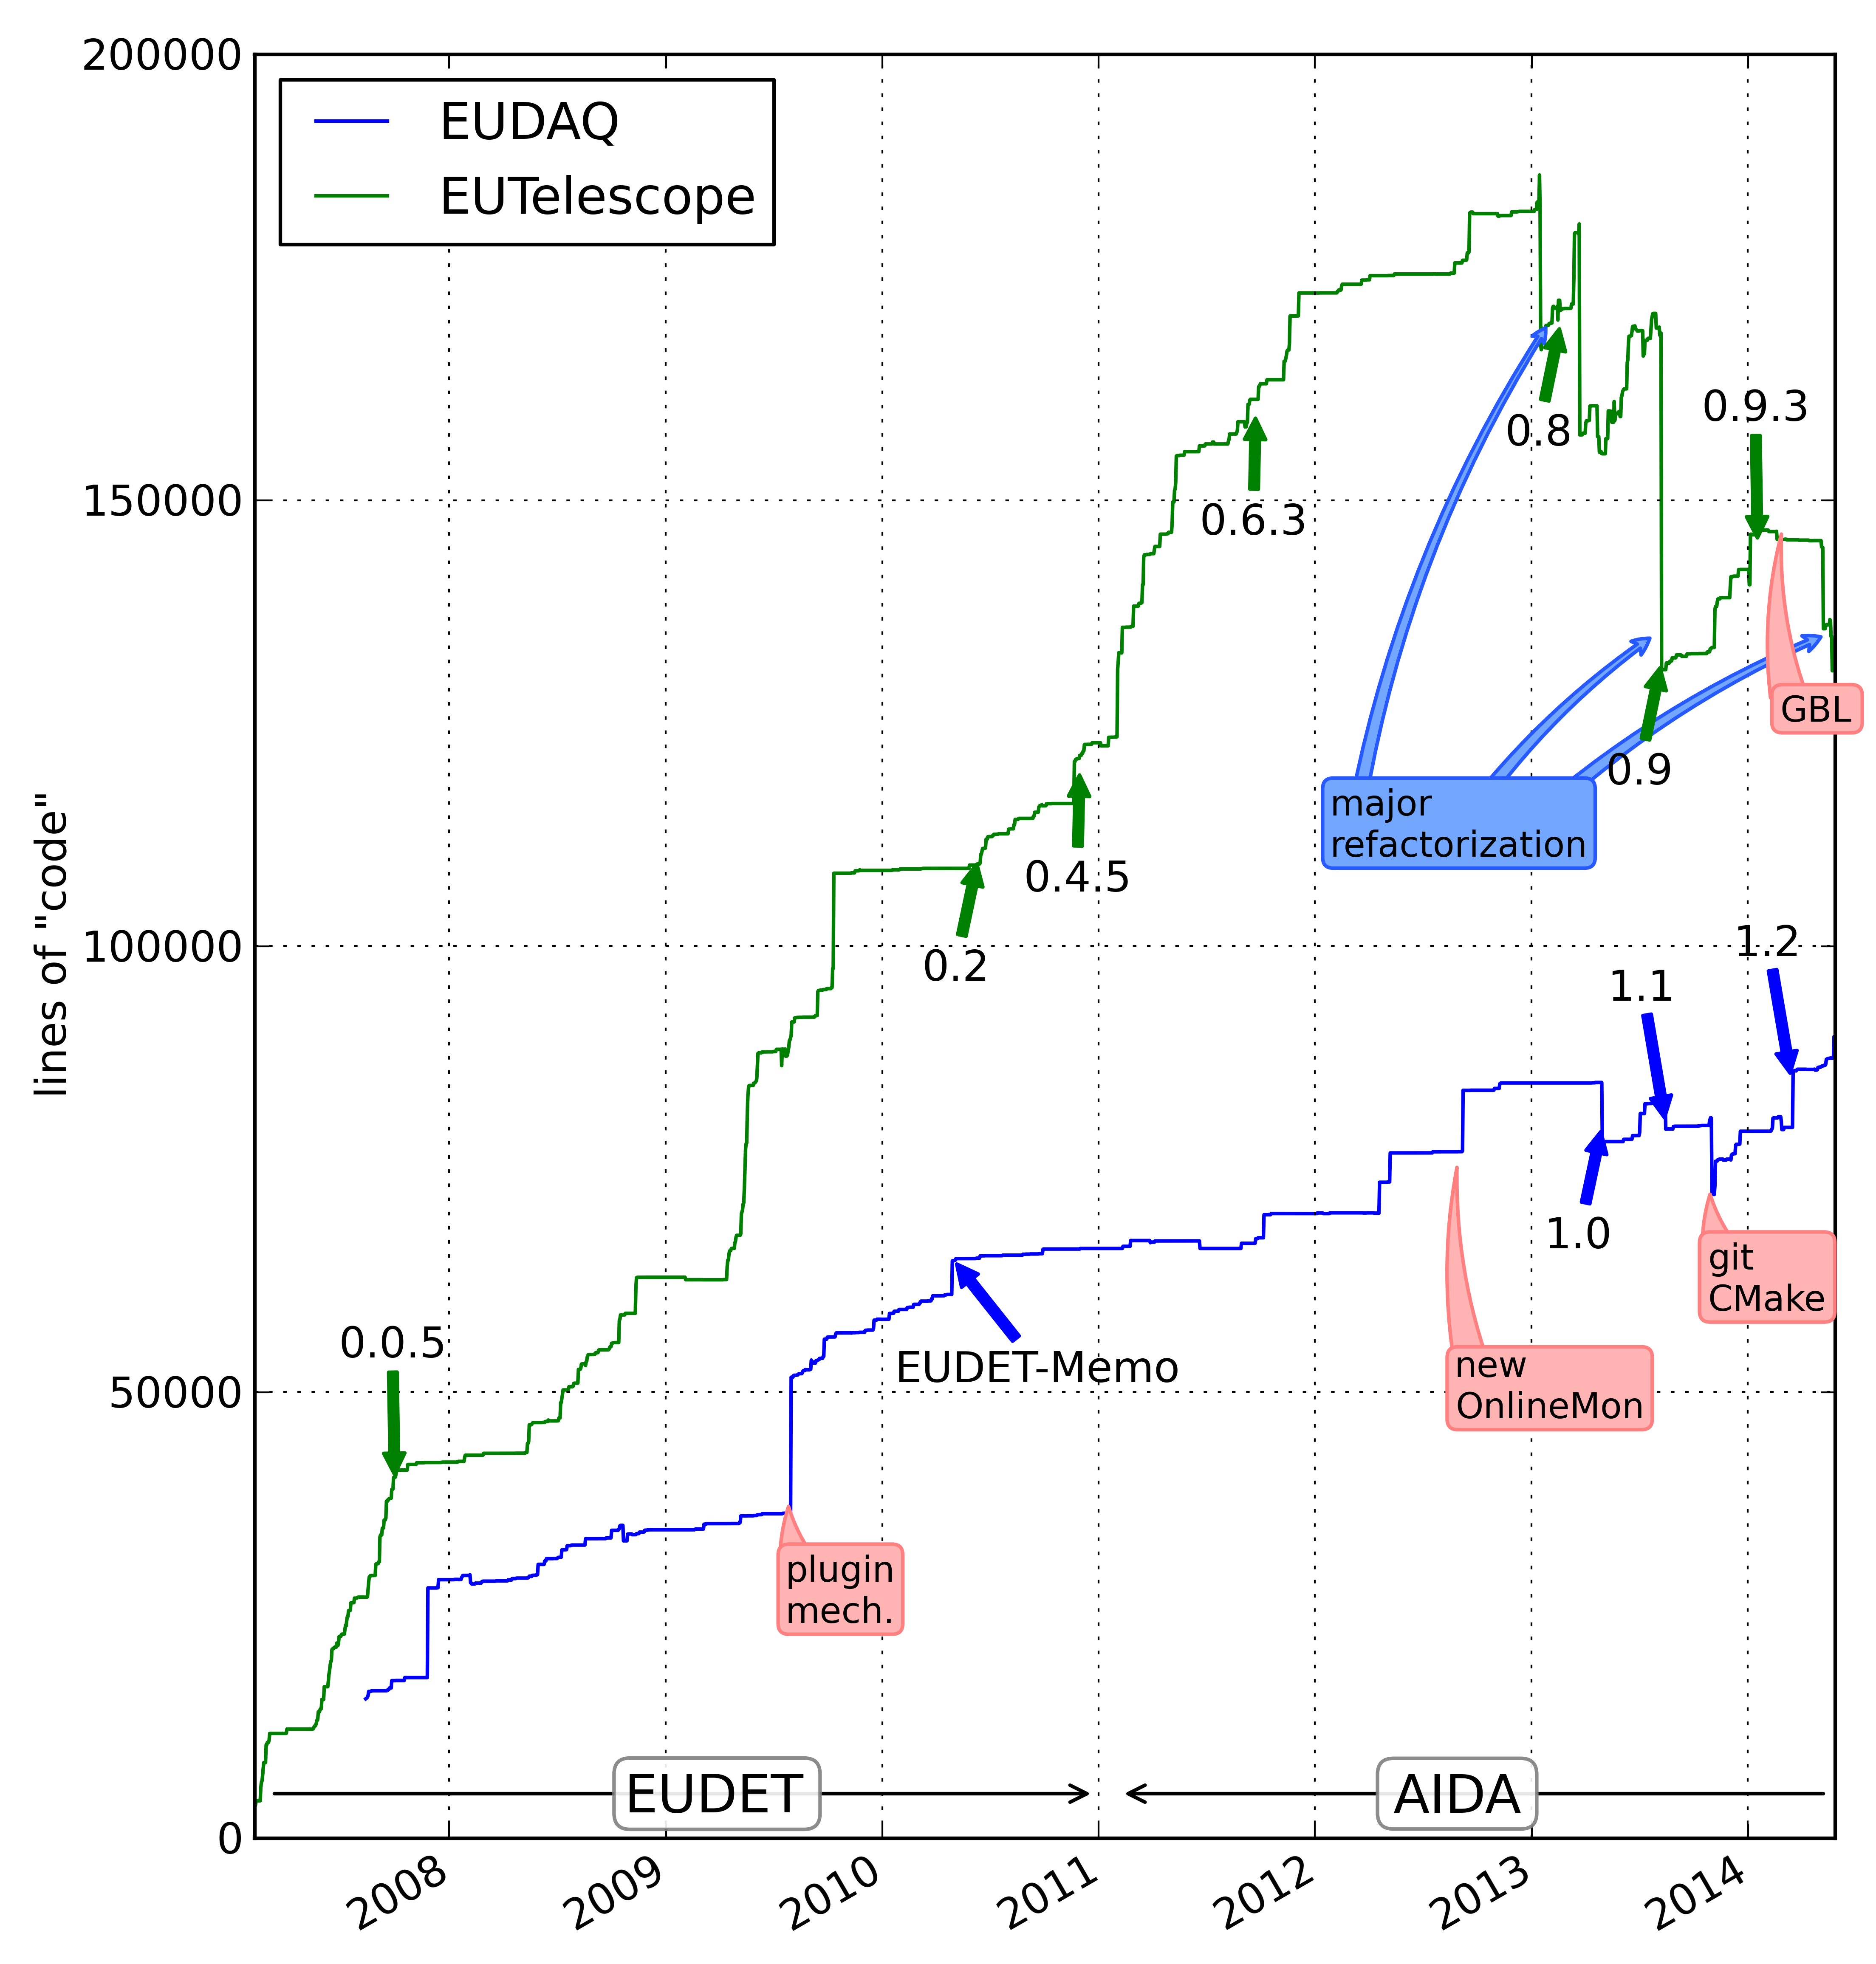
\includegraphics[width=.65\linewidth]{images/loc.png}
     \caption{Total number of lines of ``code'' (including comments,
       documentation and helper scripts) of the two software
       frameworks versus time. Selected major feature additions (red boxes),
       releases (arrows) and refactorizations (blue box) have been highlighted.}
     \label{fig:loc}
   \end{figure}

\section{Continuous Operation Needs Active Development}
With the successful usuage of the first EUDET telescope for testbeam studies since
2007, four additional copies have been produced and are being operated in
various beams around the world. This results in a constantly growing user base
with evolving needs.
These have been the focus particularly of recent releases of EUDAQ and
EUTelescope, by constantly extending the available documentation and
examples, by providing support through online forums and
workshops, and by making the installation easy and straightforward.

The quickly progressing development over the past years as illustrated
in figure~/ref{fig:loc} has been made
possible by the open development model followed for both software
frameworks which encourages external contributions. With open source
code managed through \emph{git} and hosted on GitHub, new functionality has
been integrated in close collaboration with developers from many different
institutes. Using automated nightly builds based on the CMake/CTest toolset, problems can be
identified and fixed early in the development cycle. Furthermore, data-driven regression
tests are used to constantly verify the output of the frameworks
against a set of known good references. This ensures the stability and
continued validity of the results.


\section{Summary}
EUDAQ and EUTelescope are central software components of the EUDET
beam telescopes and a key factor in their success. They offer the
user a ready-to-use framework for DAQ integration and testbeam data
analysis and are constantly being evolved to meet the user's
needs. For the next-generation AIDA telescope, both EUDAQ and
EUTelescopes are being extended to be able to cope with higher data rates, to
provide an extended data format and to handle more challenging offline
synchronization and alignment tasks.

Specifically the additional meta data available in EUDAQ will make more thorough consistency
checks and online verification possible: as devices obtain their clock
directly from the TLU, synchronization loss and missed triggers can be
reliably detected online. For this purpose, the meta data only will be
collected and verified by a central data quality monitoring
process. Additionally, the data can be (partially) merged online
by requesting packets containing specific trigger ranges -- this
allows to generate e.g. correlation plots online or even run the data
analysis on a sub-set of the data while the recording is ongoing.

Even with these fundamental changes to the data-handling concept of EUDAQ, a lot of
effort has been invested to make the modifications backward-compatible
in order to preserve existing device integrations by the users.




\section{Acknowledgments}

  The research leading to these results has received funding from the
  European Commission under the FP7 Research Infrastructures project
  AIDA, grant agreement no. 262025. The support is gratefully
  acknowledged. 
  \emph{Disclaimer}: The information herein only reflects the views of its authors and not those of the European Commission and no warranty expressed or implied is made with regard to such information or its use.

\printbibliography


%%% End document
\end{document}
